\documentclass[11pt,a4paper]{article}
\usepackage[margin=2.2cm]{geometry}
\usepackage{amsmath,amssymb}
\usepackage{booktabs}
\usepackage{array}
\usepackage{siunitx}
\usepackage{graphicx}
\usepackage[hypertexnames=false]{hyperref}
\usepackage{float}
\usepackage{enumitem}
\usepackage{xcolor}
\setlength{\emergencystretch}{8em}

\hypersetup{
  colorlinks=true,
  linkcolor=blue!50!black,
  urlcolor=blue!50!black,
  citecolor=blue!50!black
}

\title{Numerical Method Comparison for 2D Two-Target First-Passage Problem\\
\large C1 Scenario: Sparse Exact / Dense Recursion / AW (Cauchy-FFT) / Giuggioli Defect-Reduced AW / Linear Systems}
\author{valley-k-small: \texttt{reports/2d\_two\_target\_double\_peak}}
\date{2026-02-10}

\begin{document}
\sloppy
\maketitle

\begin{abstract}
This report compares five numerical routes for the same C1 setup in the 2D
two-target study: sparse exact recursion, dense recursion, Luca/Giuggioli
defect-reduced inversion, full AW/Cauchy-FFT inversion, and linear systems
for MFPT and splitting probability.
Sparse and dense recursion agree at machine precision on distribution-level
outputs, and both AW routes agree with exact recursion on their shared time
window. MFPT is still tail-sensitive, so truncated sums underestimate it,
whereas linear systems provide the most robust MFPT reference.
\end{abstract}

\section{Problem Setup}
\subsection{Targets}
We compare methods along three dimensions:
\begin{enumerate}[leftmargin=2em]
  \item \textbf{FPT distribution accuracy}: whether the method reproduces the double-peak structure and peak locations.
  \item \textbf{MFPT robustness}: whether long tails cause severe truncation bias.
  \item \textbf{Computational efficiency}: wall-clock cost at this problem size.
\end{enumerate}

\subsection{Unified C1 Configuration}
\begin{itemize}[leftmargin=2em]
  \item Grid: $N=31$, reflecting on all boundaries.
  \item Base motion: $q=0.2$ (move), $1-q=0.8$ (stay).
  \item Local bias strength: $\delta=0.2$.
  \item Start: $n_0=(14,14)$ (0-based).
  \item Targets: $m_1=(21,14)$, $m_2=(6,6)$ (0-based).
  \item Main horizon: $t_{\max}=6000$, stop threshold $S(t)<10^{-13}$.
  \item AW window: $t_{\max}^{\mathrm{AW}}=800$, oversample$=2$, $r\_\text{pow10}=8.0$, yielding $m=2048$ contour points.
\end{itemize}

\section{Unified Mathematical Framework}
\subsection{Absorbing Markov Chain Block Form}
Partition states into transient set $\mathcal T$ and absorbing set $\mathcal A=\{m_1,m_2\}$. The transition matrix is
\[
P=
\begin{pmatrix}
Q & R\\
0 & I
\end{pmatrix},\qquad
R=[r_1\ r_2].
\]
Here $Q\in\mathbb R^{|\mathcal T|\times|\mathcal T|}$ and $r_1,r_2\in\mathbb R^{|\mathcal T|}$. Let $\alpha$ be the one-hot row vector at start $n_0$.

\subsection{FPT, Survival, and MFPT Identities}
Define transient distribution
\[
u_t=\alpha Q^t.
\]
Then
\[
 f_1(t)=\alpha Q^{t-1}r_1,\quad
 f_2(t)=\alpha Q^{t-1}r_2,\quad
 f_{\mathrm{any}}(t)=f_1(t)+f_2(t).
\]
\[
S(t)=\Pr(T>t)=u_t\mathbf 1=\alpha Q^t\mathbf 1.
\]
In discrete time:
\[
 f_{\mathrm{any}}(t)=S(t-1)-S(t),\qquad
 \mathbb E[T]=\sum_{t\ge0} S(t).
\]
Hence MFPT is tail-dominated and strongly affected by truncation.

\section{Methods and Complexity}
\subsection{Method A: Sparse Exact Time Iteration}
This is the explicit probability-space recursion with target-mass extraction ("take out"):
\begin{enumerate}[leftmargin=2em]
  \item propagate one-step probabilities on the full state space;
  \item read masses landing on $m_1,m_2$ as $f_1(t),f_2(t)$;
  \item set target-site probabilities to zero;
  \item continue to the next step.
\end{enumerate}
Equivalent transient form:
\[
\nu_t=\nu_{t-1}Q,\qquad f_i(t)=\nu_{t-1}r_i.
\]
With edge-list sparse updates, per-step cost is $\mathcal O(E)$ and total cost
\[
\mathcal O(t_{\max}E),\qquad \text{memory } \mathcal O(E+N).
\]
It directly outputs the full FPT curve, but MFPT truncation can be substantial.

\subsection{Method B: Dense Recursion (Transient Space)}
Construct dense $Q$, $r_1$, $r_2$, set $\nu_0=\alpha$, and iterate
\[
\nu_t=\nu_{t-1}Q,\quad f_i(t)=\nu_{t-1}r_i,\quad f_{\mathrm{any}}(t)=f_1(t)+f_2(t).
\]
Mathematically equivalent to Method A, but with dense matrix operations.
For $n_T:=|\mathcal T|$:
\[
\mathcal O(t_{\max}n_T^2),\qquad \text{memory } \mathcal O(n_T^2).
\]
This is mainly a correctness baseline.

\subsection{Method C: Luca/Giuggioli Defect-Reduced AW Inversion (Implemented)}
This is the transform-domain route used to realize Luca/Giuggioli-style defect reduction in this project.

\textbf{Step C1: defect decomposition.}
Represent the transient operator as
\[
Q=Q_0+\sum_{e=1}^{M}\delta_e\,\mathbf e_{u_e}\mathbf e_{v_e}^{\top}
=Q_0+U\Delta V^\top,
\]
where $Q_0$ is a solvable baseline, $M$ is the number of defect pairs, and
$\Delta=\mathrm{diag}(\delta_1,\dots,\delta_M)$.

\textbf{Step C2: selected propagator via Woodbury.}
For a complex point $z$ and baseline Green matrix
\[
P^0(z):=(I-zQ_0)^{-1},
\]
define $S=\{s,m_1,m_2\}$ and $T=\{m_1,m_2\}$. The required entries are
\[
P_{S,T}(z)
=P^0_{S,T}(z)
+z\,P^0_{S,U}(z)\,\Delta
\bigl[I_M-z\,P^0_{V,U}(z)\,\Delta\bigr]^{-1}
P^0_{V,T}(z).
\]
So each $z$-point uses an $M\times M$ defect solve instead of a full $n_T\times n_T$ solve.

\textbf{Step C3: two-target renewal closure.}
Using the selected propagators,
\[
\begin{bmatrix}
P_{s,m_1}(z)\\
P_{s,m_2}(z)
\end{bmatrix}
=
\begin{bmatrix}
P_{m_1,m_1}(z) & P_{m_2,m_1}(z)\\
P_{m_1,m_2}(z) & P_{m_2,m_2}(z)
\end{bmatrix}
\begin{bmatrix}
F_1(z)\\
F_2(z)
\end{bmatrix},
\]
hence $F(z)=G(z)^{-1}b(z)$ is solved from a $2\times2$ system at each $z$.

\textbf{Step C4: FFT coefficient recovery.}
Sample on $z_k=r e^{i2\pi k/m}$ and invert:
\[
 f_i(t)\approx r^{-t}\cdot\frac{1}{m}\sum_{k=0}^{m-1}F_i(z_k)e^{-i2\pi kt/m}.
\]

Complexity:
\[
\mathcal O\!\big(m\,[C_{\text{base}}(n_T)+M^3]+m\log m\big),
\]
where $C_{\text{base}}(n_T)$ is baseline Green-evaluation cost on selected node sets.
In this project this method is implemented and benchmarked using defect-pair matrices.

\subsection{Method C0: Full AW / Cauchy-FFT (Dense Baseline)}
For comparison, full AW directly uses
\[
\tilde f_i(z)=z\,\alpha\,(I-zQ)^{-1}r_i,
\]
with one full $n_T\times n_T$ complex solve per contour point.
Its cost is
\[
\mathcal O(mn_T^3 + m\log m),\qquad \text{memory } \mathcal O(n_T^2+m).
\]
In this report full AW is used on $t\le 800$ as a transform-domain baseline.

\subsection{Method D: Linear Systems (MFPT / Splitting)}
Solve moments directly instead of the full distribution:
\[
(I-Q)m=\mathbf 1,\qquad (I-Q)u_i=r_i.
\]
At $n_0$:
\[
\mathrm{MFPT}=m(n_0),\qquad p_i=u_i(n_0),\qquad p_1+p_2=1.
\]
With dense direct solve:
\[
\mathcal O(n_T^3),\qquad \text{memory } \mathcal O(n_T^2).
\]
This is the most robust route when MFPT/splitting are the primary outputs.

\section{Complexity Table}
\begin{table}[H]
  \centering
  \small
  \begin{tabular}{>{\raggedright\arraybackslash}p{3.3cm}>{\raggedright\arraybackslash}p{5.8cm}>{\raggedright\arraybackslash}p{3.8cm}}
    \toprule
    Method & Time complexity (dominant term) & Memory complexity \\
    \midrule
    Sparse exact recursion & $\mathcal O(t_{\max}E)$ & $\mathcal O(E+N)$ \\
    Dense recursion ($Q$) & $\mathcal O(t_{\max}n_T^2)$ & $\mathcal O(n_T^2)$ \\
    Luca defect-reduced AW (Method C) & $\mathcal O(m[C_{\text{base}}(n_T)+M^3]+m\log m)$ & $\mathcal O(M^2+n_T)$ to $\mathcal O(n_T^2)$ \\
    Full AW/Cauchy-FFT (Method C0) & $\mathcal O(mn_T^3 + m\log m)$ (dense solve) & $\mathcal O(n_T^2+m)$ \\
    Linear systems (MFPT/splitting) & $\mathcal O(n_T^3)$ (dense solve) & $\mathcal O(n_T^2)$ \\
    \bottomrule
  \end{tabular}
  \caption{Complexity summary. Symbols: $N$ total states, $E$ effective edges, $n_T=|\mathcal T|$, $m$ inversion sample points.}
\end{table}

\subsection{Scale Instantiation for C1}
In this setup:
\[
N=31^2=961,\quad n_T=959,\quad E\approx4681,\quad m=2048.
\]
So:
\begin{itemize}[leftmargin=2em]
  \item sparse exact scales roughly with $t_{\max}\times4.7\times10^3$;
  \item dense recursion scales with $t_{\max}\times9.2\times10^5$;
  \item full AW (Method C0) includes about $m$ full complex linear solves;
  \item for implemented defect-reduced AW in C1:
  \[
  M_{\text{pairs}}=632,\quad M_{\text{nodes}}=326,\quad M_{\text{local-bias-sites}}=317;
  \]
  \item with pair-level reduction ($M=632$), solve-core reduction estimate is
  \[
  (n_T/M)^3=(959/632)^3\approx3.5\times
  \]
  (or $(959/632)^{2.81}\approx3.2\times$ under exponent $2.81$);
  \item linear systems are most cost-effective for MFPT/splitting-only goals.
\end{itemize}

\subsection{Literature-Notation Consistency}
To avoid notation mismatch, we map symbols as follows:
$N^d$ in lattice papers corresponds to state-space scale (here comparable to $n_T$),
while $M$ denotes defect support size under a chosen defect representation.
In Sarvaharman--Giuggioli (Phys.\ Rev.\ Research 5, 013118, Sec.\ V), the explicit
first-passage route is reported with scaling $\mathcal O(M^2N^d)$, while brute-force
time stepping is reported as $\mathcal O(N^{2d}t)$ (or with a fast matrix exponent
$2.373d$ in the same discussion). The older $2.81$ exponent used in some reports
comes from the Strassen-style dense exponent model. Different exponents therefore
reflect different linear-algebra assumptions, not a contradiction in method structure.

\section{Measured Results}
\subsection{Runtime}
\begin{table}[H]
  \centering
  \begin{tabular}{lc}
    \toprule
    Method & Runtime (s) \\
    \midrule
    Sparse exact recursion & 0.0561 \\
    Dense recursion ($Q$) & 0.0919 \\
    Luca defect-reduced AW (Method C) & 78.0223 \\
    Full AW/Cauchy inversion (Method C0) & 47.2622 \\
    Linear systems (MFPT/splitting) & 0.0213 \\
    \bottomrule
  \end{tabular}
  \caption{Wall-clock comparison on C1.}
\end{table}

\subsection{Distribution Errors (Sparse Exact as Baseline)}
\begin{table}[H]
  \centering
  \begin{tabular}{lcc}
    \toprule
    Comparison & $L^1$ error & $L^\infty$ error \\
    \midrule
    Dense vs Sparse (common horizon) & $9.212\times10^{-15}$ & $1.924\times10^{-18}$ \\
    Luca-defect (C) vs Sparse ($1..t_{\max}^{\mathrm{AW}}$) & $9.912\times10^{-10}$ & $1.426\times10^{-12}$ \\
    Full AW (C0) vs Sparse ($1..t_{\max}^{\mathrm{AW}}$) & $9.912\times10^{-10}$ & $1.426\times10^{-12}$ \\
    \bottomrule
  \end{tabular}
  \caption{Dense and sparse agree at machine precision; both transform routes are highly accurate on the shared window.}
\end{table}

\subsection{Key Statistics}
\begin{table}[H]
  \centering
  \small
  \begin{tabular}{lcccccc}
    \toprule
    Method & mass\_any & tail & MFPT (trunc./exact) & peak1 & peak2 \\
    \midrule
    Sparse exact ($t\le 6000$) & 0.850786 & 0.149214 & 1583.479 & 35 & 284 \\
    Sparse exact ($t\le 800$) & 0.297030 & 0.702970 & 111.653 & 35 & 284 \\
    Dense recursion ($t\le 6000$) & 0.850786 & 0.149214 & 1583.479 & 35 & 284 \\
    Luca defect-reduced ($t\le 800$) & 0.297030 & 0.702970 & 111.653 & 35 & 284 \\
    Full AW inversion ($t\le 800$) & 0.297030 & 0.702970 & 111.653 & 35 & 284 \\
    Linear systems (full-time) & 1.000000 & 0.000000 & 3011.214 & - & - \\
    \bottomrule
  \end{tabular}
  \caption{Luca-defect and full AW are both identical to sparse exact on $t\le 800$. Long-tail mass dominates MFPT.}
\end{table}

\subsection{Defect Scale and Practical Impact (C1)}
\begin{itemize}[leftmargin=2em]
  \item Defect profile in this implementation: local-bias sites $=317$, defect pairs $=632$, defect nodes $=326$.
  \item Measured runtime on C1: Luca-defect (Method C) is slower ($78.0$s) than full AW baseline (Method C0, $47.3$s).
  \item Interpretation: at this defect size, solve-core reduction alone is insufficient to offset baseline Green-function and assembly overhead.
  \item Practical takeaway: defect reduction becomes advantageous when defect support is much sparser ($M\ll n_T$) or when the implementation further compresses defect dimension.
\end{itemize}

\subsection{MFPT Truncation Bias}
\begin{table}[H]
  \centering
  \small
  \begin{tabular}{ccccc}
    \toprule
    $t_{\max}$ & absorbed mass & tail mass & truncated MFPT & relative error (vs linear systems) \\
    \midrule
    300 & 0.116714 & 0.883286 & 19.294 & -99.359\% \\
    600 & 0.241807 & 0.758193 & 73.099 & -97.572\% \\
    1200 & 0.389579 & 0.610421 & 203.559 & -93.240\% \\
    2400 & 0.581766 & 0.418234 & 540.034 & -82.066\% \\
    6000 & 0.850786 & 0.149214 & 1583.479 & -47.414\% \\
    \bottomrule
  \end{tabular}
  \caption{MFPT is strongly tail-driven; truncation yields systematic underestimation.}
\end{table}

\subsection{Constructed Luca-Fast Case (LF1)}
To explicitly answer when Luca/Giuggioli defect reduction can be the fastest route, we constructed an ultra-sparse defect case (single local-bias site) and benchmarked all methods:
\[
N=41,\quad n_T=1679,\quad t_{\max}=12000,\quad t_{\max}^{\mathrm{AW}}=80,\quad M_{\text{pairs}}=2.
\]
\begin{table}[H]
  \centering
  \begin{tabular}{lc}
    \toprule
    Method & Runtime (s) \\
    \midrule
    Luca/Giuggioli defect-reduced (Method C) & 0.0198 \\
    Linear systems (MFPT/splitting) & 0.0477 \\
    Sparse exact recursion & 0.1754 \\
    Dense recursion ($Q$) & 1.6187 \\
    Full AW/Cauchy (Method C0) & 22.8746 \\
    \bottomrule
  \end{tabular}
  \caption{LF1: Luca method is the fastest in this constructed regime.}
\end{table}
\begin{figure}[H]
  \centering
  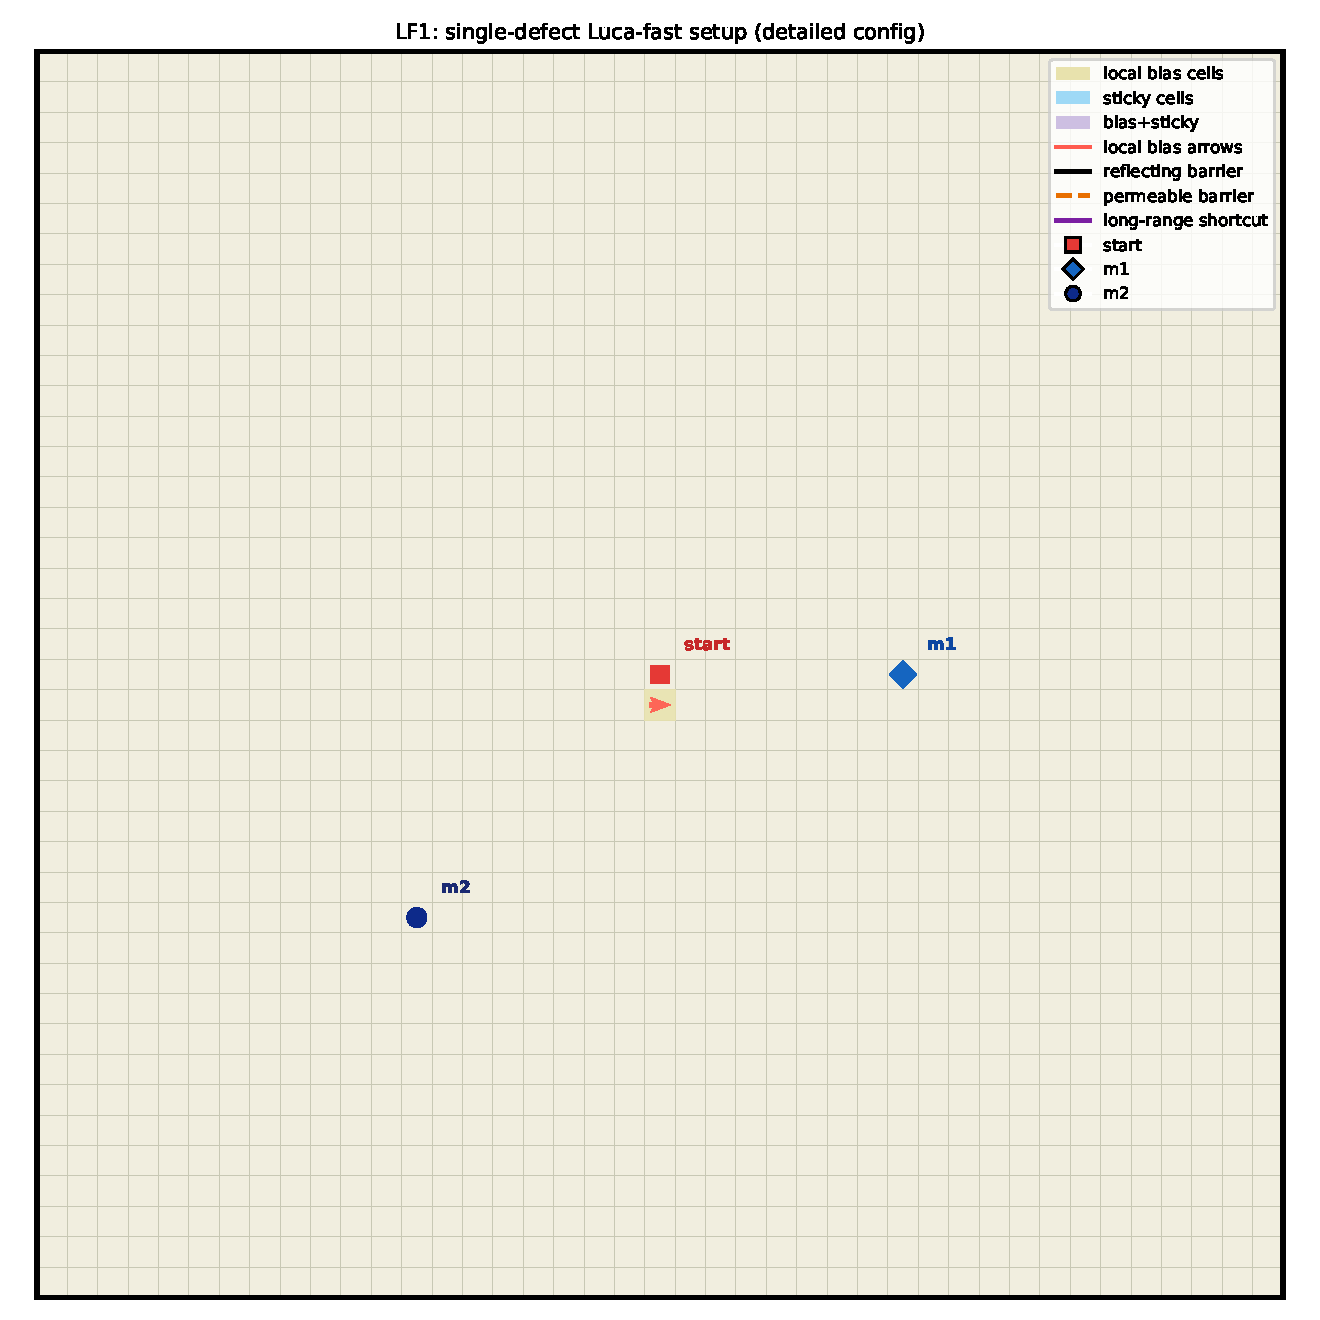
\includegraphics[width=0.78\linewidth]{figures/luca_fast_case_config_detailed.pdf}
  \caption{LF1 configuration (same visual style as the external detailed-config panels).}
\end{figure}
\begin{figure}[H]
  \centering
  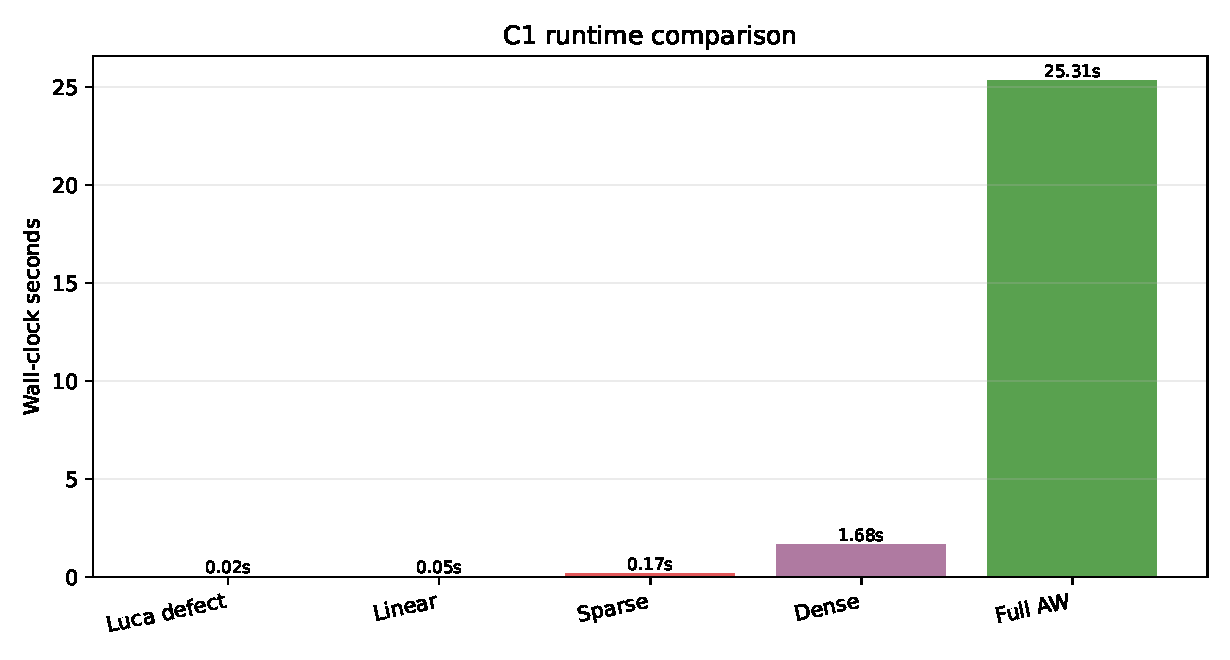
\includegraphics[width=0.88\linewidth]{figures/luca_fast_case_runtime.pdf}
  \caption{LF1 runtime comparison.}
\end{figure}
The mechanism is direct: with $M=2$, Method C solves a tiny defect system while full AW and dense baselines still carry large linear-algebra kernels.

\section{Figures}
\begin{figure}[H]
  \centering
  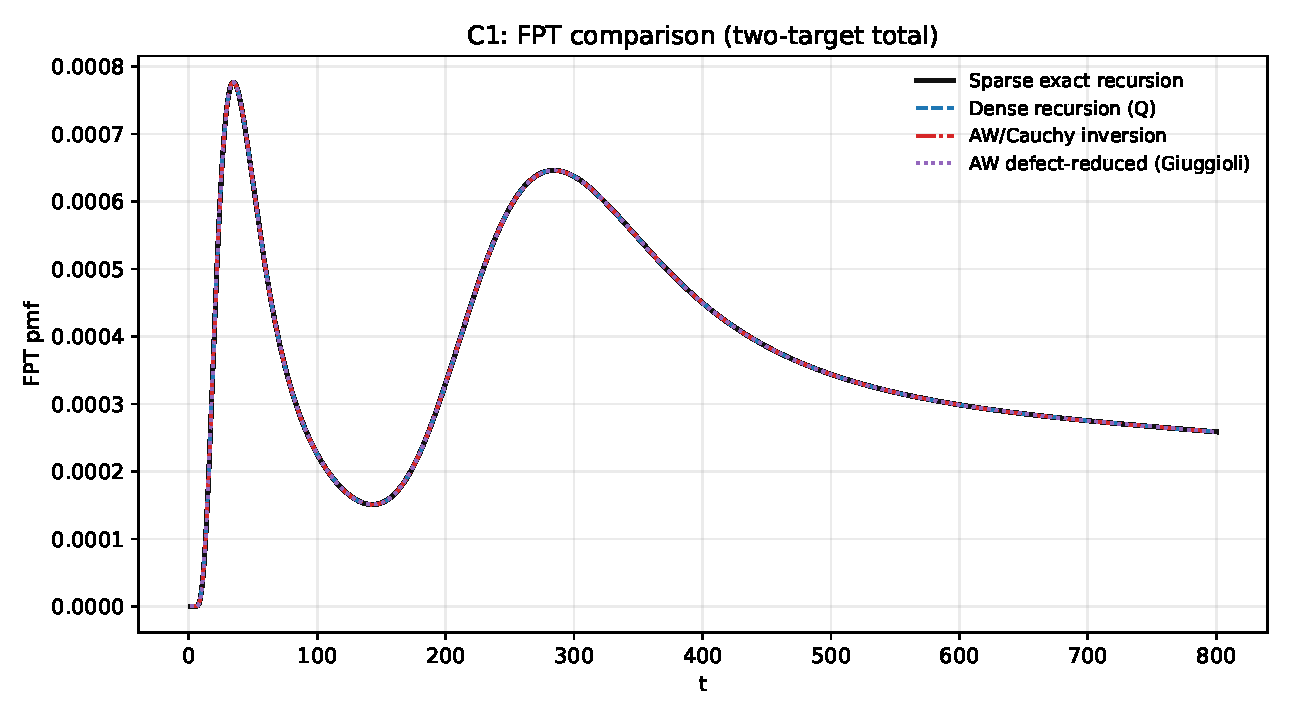
\includegraphics[width=0.95\linewidth]{figures/method_compare_c1_fpt_overlay.pdf}
  \caption{FPT overlays: Sparse / Dense / Luca-defect / Full AW (nearly identical on shared horizon).}
\end{figure}

\begin{figure}[H]
  \centering
  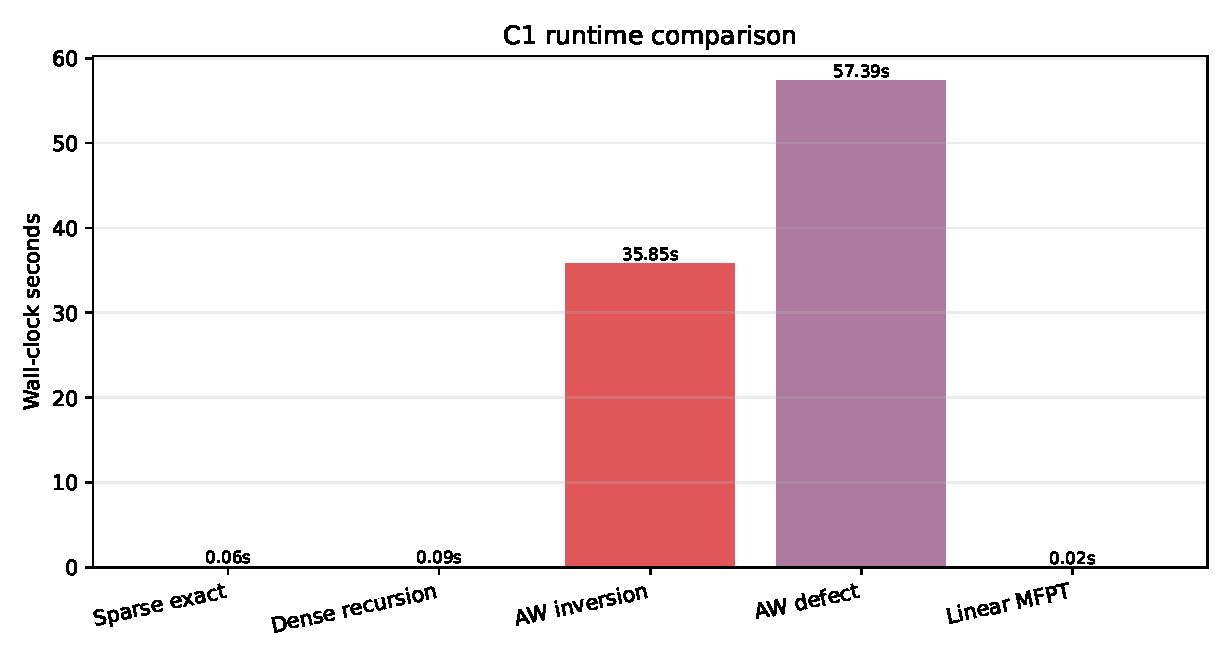
\includegraphics[width=0.88\linewidth]{figures/method_compare_c1_runtime.pdf}
  \caption{Runtime comparison.}
\end{figure}

\section{Conclusions and Recommendations}
\begin{enumerate}[leftmargin=2em]
  \item \textbf{Need full double-peak FPT curves}: use sparse exact recursion.
  \item \textbf{Need robust MFPT/splitting}: use linear systems; avoid relying on truncated sums.
  \item \textbf{Method C (Luca-defect)}: mathematically explicit and accurate; in this C1 setup it is slower than full AW because defect support is not small enough.
  \item \textbf{Need transform-domain analysis}: use full AW as direct baseline and switch to Method C when defect support is truly sparse ($M\ll n_T$) and overhead is controlled.
\end{enumerate}

\section*{Reproduction}
\texttt{.venv/bin/python reports/2d\_two\_target\_double\_peak/code/compare\_numeric\_methods.py}

\end{document}
